
\documentclass[a4paper,11pt]{article}
%%%%%%%%%%%%%%%%%%%%%%%%%%%%%%%%%%%%%%%%%%%%%%%%%%%%%%%%%%%%%%%%%%%%%%%%%%%%%%%%%%%%%%%%%%%%%%%%%%%%%%%%%%%%%%%%%%%%%%%%%%%%%%%%%%%%%%%%%%%%%%%%%%%%%%%%%%%%%%%%%%%%%%%%%%%%%%%%%%%%%%%%%%%%%%%%%%%%%%%%%%%%%%%%%%%%%%%%%%%%%%%%%%%%%%%%%%%%%%%%%%%%%%%%%%%%
\usepackage{amsfonts}
\usepackage{amsmath}
\usepackage{natbib}
\usepackage{graphicx}
\usepackage{booktabs}
\usepackage[onehalfspacing]{setspace}


\graphicspath{ {images/} }
\setcounter{MaxMatrixCols}{10}
%TCIDATA{OutputFilter=LATEX.DLL}
%TCIDATA{Version=5.50.0.2960}
%TCIDATA{<META NAME="SaveForMode" CONTENT="1">}
%TCIDATA{BibliographyScheme=Manual}
%TCIDATA{Created=Wednesday, March 01, 2017 12:55:57}
%TCIDATA{LastRevised=Monday, August 14, 2017 13:56:18}
%TCIDATA{<META NAME="GraphicsSave" CONTENT="32">}
%TCIDATA{<META NAME="DocumentShell" CONTENT="Standard LaTeX\Blank - Standard LaTeX Article">}
%TCIDATA{CSTFile=40 LaTeX article.cst}

\newtheorem{theorem}{Theorem}
\newtheorem{acknowledgement}[theorem]{Acknowledgement}
\newtheorem{algorithm}[theorem]{Algorithm}
\newtheorem{axiom}[theorem]{Axiom}
\newtheorem{case}[theorem]{Case}
\newtheorem{claim}[theorem]{Claim}
\newtheorem{conclusion}[theorem]{Conclusion}
\newtheorem{condition}[theorem]{Condition}
\newtheorem{conjecture}[theorem]{Conjecture}
\newtheorem{corollary}[theorem]{Corollary}
\newtheorem{criterion}[theorem]{Criterion}
\newtheorem{definition}[theorem]{Definition}
\newtheorem{example}[theorem]{Example}
\newtheorem{exercise}[theorem]{Exercise}
\newtheorem{lemma}[theorem]{Lemma}
\newtheorem{notation}[theorem]{Notation}
\newtheorem{problem}[theorem]{Problem}
\newtheorem{proposition}[theorem]{Proposition}
\newtheorem{assumption}{Assumption}
\newtheorem{remark}[theorem]{Remark}
\newtheorem{solution}[theorem]{Solution}
\newtheorem{summary}[theorem]{Summary}
\newenvironment{proof}[1][Proof]{\noindent\textbf{#1.} }{\ \rule{0.5em}{0.5em}}
\newcommand{\argmax}{\operatornamewithlimits{argmax}}

\begin{document}

\title{Equilibrium trip scheduling and mode choice in the ride-sourcing problem under travel time uncertainty }
\author{Zheng Liang\thanks{Hong Kong University of Science and Technology}
\and
Gege Jiang\thanks{Corresponding: Hong Kong University of Science and Technology, gjiang@ust.hk}
\and
Hong K. Lo \thanks{Hong Kong University of Science and Technology}}
\maketitle

\begin{abstract}
This paper 
\end{abstract}

\noindent Keywords: mode choice; departure time ;ride-sourcing; random delay; bottleneck

\bigskip
\section{introduction}
\section{Problem formulation}\label{sec:model}

The problem is defined for $N$ travelers commuting between home and work daily during morning peak hours with the same preferred arrival time $t^*$. In this study, commuters are considered to choose among four modes: 1) driving on their own, 2) taking non-shared service, 3) taking ride-sharing service and 4) metro. 

The commuters of the first three travel modes have to travel through a single bottleneck with a deterministic discharging rate $s$. In addition to the free-flow travel time $T_0$ and queuing time $Q(t)$ of the bottleneck, all of them are susceptible to an exogenous random travel delay $R$, which is upper-bounded by $\overline{t}$ and lower-bounded by $0$.
\textbf{(You should add an explanation what is the source of random delay. Cite some paper and state it clearly.)} The probability distribution of $R$ is known to all travelers. Affecting all the commuters in the same way, $R$ takes on a different realization $r$ from day to day, but remains the same in a day. Meanwhile, commuters of the last travel mode do not experience travel time variability, their travel time $T_{mtr}$ is fixed.

\subsection{Notations} \label{subs:notation}

The parameters and variables in this paper are shown in the following table.

\begin{table}[htbp]
 \caption{List of parameters and variables \label{tab:variables}}
 \begin{center}
 \begin{tabular}{cl}
 
  \toprule
   Parameter & Definition   \\
  \midrule
 $\alpha$ & value of time \\
 $\beta$ & value of early delay  \\
 $\gamma$ & value of late delay   \\
 $\mu_i$ & time unit price of mode $i$ \\
 $t^*$ & preferred arrival time  \\
 $\overline{t}$ & upper-bound of random travel delay  \\
 $T_0$ & free flow travel time \\
 $s$ & service rate of the bottleneck \\

  \bottomrule
\cr
    \toprule
   Variable & Definition   \\
  \midrule
 $q_{i,j}(t)$ & queuing rate of mode $i$ and type $j$ commuters at time $t$ \\
 $Q_{i,j}(t)$ & queue length of mode $i$ and type $j$ commuters at time $t$ \\
 $N_i$ & number of commuters of each travel mode ($i=1,2,3,4$) \\
 $\overline{N}$ & number of operating vehicles on road \\
 $GC_i$ & general cost of mode $i$ commuters \\
 
  \bottomrule
  
 \end{tabular}
 \end{center}
\end{table}


\subsection{Main assumptions} \label{subs:main assumptions}

Before proposing the model framework, the main assumptions are mentioned here.

\begin{assumption} \label{ass:same value of time}
All the $N$ commuters are with homogeneous parameters in terms of value of time $\alpha$, value of schedule early delay $\beta$, and value of schedule late delay $\gamma$, and $\alpha>\beta$.
\end{assumption}

As proved in \cite{lindsey2004existence}, the existence of equilibrium requires $\alpha>\beta$, yielding the growing queue for early arrivals. The assumption of homogeneous is adopted by many previous studies (e.g. \cite{wang2016equilibrium}; \cite{liu2017pricing}).

\begin{assumption} \label{ass:uniform distribution}
The random travel delay $R$ follows a uniform distribution, $R\sim U[0,\overline{t}]$, and the probability density is $f(r)=\frac{1}{\overline{t}}$. The same assumption is imposed by \cite{siu2009equilibrium}.
\end{assumption}


\begin{assumption} \label{ass:two in ride-sharing}
There are and only are two passengers sharing in one single vehicle of the ride-sharing service during the morning peak period.
\end{assumption}

The ride-sharing service, including the car and driver, is provided by the TNCs. The ride-sharing vehicle capacity is limited, and for simplicity we assume the number of passengers in each trip is two.

\begin{assumption} \label{ass:positive MTR}
Metro is always chosen by certain commuters during the morning peak period, and its general cost is fixed.
\end{assumption}

No travel delay or congestion is included in metro, so the travel time $T_{MTR}$ is relatively fixed. Besides, the metro ticket fare from home to work $C_{MTR}$ is also fixed and given. So the general cost by metro $GC_4$ is deterministic, i.e.
\begin{equation*}
    GC_4=\alpha T_{MTR} + C_{MTR} = GC_{MTR}
\end{equation*}

In reality, metro is always an active mode choice among commuters. With this assumption, the general cost of the metro can be treated as a benchmark in our problem, since all commuters have identical cost in the equilibrium.

\subsection{Schedule delay} \label{subsec:Schedule delay}

 According to \cite{small1982scheduling}, schedule delay is defined as the time gap between the work start time $t^*$ and their actual arrival time, and it can be classified into Schedule Delay Early (SDE) for early arrivals and Schedule Delay Late (SDL) for late arrivals:

\begin{equation} 
SDE\left(t\right)=max \left\{t^*-\left(t+T_0+\frac{Q(t)}{s}+r\right), 0\right\}
\label{SDE}
\end{equation}

\begin{equation} 
SDL\left(t\right)=max \left\{0, \left(t+T_0+\frac{Q(t)}{s}+r\right)-t^*\right\}
\label{SDL}
\end{equation}

In the morning peak period, some road users, departing early enough, will arrive at their workplaces before the work start time $t^*$ even though they experience the maximum travel delay $\overline{t}$. On the contrary, others must be late for work even if they go through 0 random delay. So in the expressions below, we define $t_e$ and $t_l$ as the two moments that departures before $t_e$ must early arrivals and departures after $t_l$ must be late arrivals.

\begin{equation}
\left\{
\begin{array}{l}
t_e=t^*-\left(T_0+\frac{Q(t_e)}{s}+\overline{t}\right)  \\
t_l=t^*-\left(T_0+\frac{Q(t_l)}{s}\right)
\end{array}
\right.  \label{tetl}
\end{equation}

Besides, commuters departing between time $t_e$ and $t_l$ are not sure whether they arrive early or late at work. Based on their on-time arrival status, all the morning commuters can be classified into three types ($j=1,2,3$), as shown in Table \ref{tab:three type commuters}.

\begin{table}[htbp]
 \caption{Three types of commuters \label{tab:three type commuters}}
 \begin{center}
 \begin{tabular}{ccc}
 
  \toprule
   Type ($j$) & Departure time $t$ & On-time arrival status \\
  \midrule
 $j=1$ & $t \leq t_e$ & early arrival \\
 $j=2$ & $t_e < t < t_l$ & early or late \\
 $j=3$ & $t \geq t_l$ & late arrival \\

  \bottomrule

 \end{tabular}
 \end{center}
\end{table}

Following equations \ref{SDE} and \ref{SDL}, which shows the schedule delay in an exact day, we take the expectation to derive SDE and SDL for a long term period:

\begin{equation}
E\left[SDE(t)\right]=\int^{max \left\{0, \left(t+T_0+\frac{Q(t)}{s}\right)-t^*\right\}}_0
\left[t^*-\left(t+T_0+\frac{Q(t)}{s}+r\right) \right]f(r)dr
\label{ESDE}
\end{equation}

\begin{equation}
E\left[SDL(t)\right]=\int^{\overline{t}}_{max \left\{0, \left(t+T_0+\frac{Q(t)}{s}\right)-t^*\right\}} 
\left[\left(t+T_0+\frac{Q(t)}{s}+r\right)-t^*\right]f(r)dr
\label{ESDL}
\end{equation}

Results are listed in Table \ref{tab:schedule delay} with .

\begin{table}[htbp]
 \caption{Expressions for schedule delay, for $R\sim U[0,\overline{t}]$ \label{tab:schedule delay}}
 \begin{center}
 \begin{tabular}{lcc}
 
  \toprule
   Type ($j$) & $E[SDE(t)]$ & $E[SDL(t)]$   \\
  \midrule
 $j=1$ & $t^*-\left(T_0+\frac{Q(t)}{s}+t+\frac{\overline{t}}{2} \right)$ & 0 \\
 $j=2$ & $ \frac{\left[ t^*-\left(T_0+\frac{Q(t)}{s}+t \right) \right]^2}{2\overline{t}} $ & $\frac{\left[ \left(T_0+\frac{Q(t)}{s}+t+\overline{t} \right)-t^* \right]^2}{2\overline{t}}$ \\
 $j=3$ & 0 &  $\left(T_0+\frac{Q(t)}{s}+t+\frac{\overline{t}}{2} \right)-t^*$ \\
  \bottomrule
  
 \end{tabular}
 \end{center}
\end{table}



\subsection{General Cost} \label{subsec:General cost}

Basically, the general cost for commuters are different depending on their travel mode choice. For commuters of the first three modes, the general cost consists of three components, i.e. 1) in-vehicle travel time consumption, 2) schedule delay penalty and 3) mode-specific expense. The  first component is a time related term, upon the total travel time $T$ ($T=T_0+\frac{Q(t)}{s}+R$); the second term depends on their on-time arrival status and the relative schedule delay and the last term is different among three modes.

For drivers (mode 1), the mode-specific expense consists of two terms: 1) a time-related cost $\mu_1E[T]$, seen as gasoline consumption and 2) a fixed cost $\delta$, inclusive of vehicle depreciation cost and parking fee. So, the general cost of them is:

\begin{equation}
    GC_1=\alpha E[T]+\beta E[SDE(t)]+\gamma E[SDL(t)]+ \delta +\mu_1 E[T]
\end{equation}

For non-sharing service users (mode 2), the mode-specific expense is a time-related cost $\mu_2E[T]$, which passengers should pay for the taxi driver according to the actual travel time. Then the general cost of them is:

\begin{equation}
    GC_2=\alpha E[T]+\beta E[SDE(t)]+\gamma E[SDL(t)] +\mu_2 E[T]
\end{equation}

For ride-sharing service users (mode 3), the mode-specific expense can be separated into two components: 1) a time-related inconvenience cost $\mu_3 E[T]$ and 2) a deterministic tour cost $\tau$. The inconvenience cost can be interpreted as the cost of uncomfortable staying in vehicle with other passengers. Longer the time they stay, more uncomfortable they will feel. 
In ride-sharing service, provided by TNCs, each passenger should pay a fixed amount of tour cost $\tau$ to the platform. So, the general cost of them is:

\begin{equation}
    GC_3=\alpha E[T]+\beta E[SDE(t)]+\gamma E[SDL(t)]+\tau +\mu_3 E[T]
\end{equation}

In the general cost functions above, known that both the first and the last term are related to the total travel time $T$. Then we define $\alpha+\mu_i \quad (i=1,2,3)$ as the composite value of time (CVoT). Although all commuters are homogeneous with respect to their value of time, their CVoT is not the same among different travel modes. But it still remains identical within one single mode. Before proceeding, we make an extra assumption of their CVoT relation:

\begin{assumption} \label{ass:mu relation}
The relationship of time unit pricing parameters in mode-specific expense is: $\mu_2>\mu_1>\mu_3$.
\end{assumption}

Generally, the time-related cost for non-sharing users consists of fuel cost used and labor cost for driver while drivers only pay for fuel cost, so $\mu_2$ is higher than $\mu_1$. As for ride-sharing service users, that is the inconvenience cost, which is considered relatively low compared to other modes. So we think the time-related cost of them is the cheapest among all three. 


Then based on the results from Table \ref{tab:schedule delay}, we can further derive the general cost functions of the first three modes in different types:

\begin{equation}
    GC_{1,j}=\left\{ 
    \begin{array}{l}
\left(\alpha+\mu_1-\beta \right)\left(T_0+\frac{Q_{1,j}(t)}{s}+\frac{\overline{t}}{2} \right)+\beta \left(t^*-t \right)+\delta, \quad j=1 \\
\left(\frac{\beta+\gamma}{2\overline{t}s^2} \right)\left[Q_{1,j}(t)-s(t^*-t) \right]^2+\left(\alpha+\mu_1+\gamma \right)\left[T_0+\frac{Q_{1,j}(t)}{s}+\frac{\overline{t}}{2} \right] \cr
+T_0\left(\frac{\beta+\gamma}{\overline{t}} \right)\left[\frac{T_0}{2}-(t^*-t)+\frac{Q_{1,j}(t)}{s} \right]+\gamma(t-t^*)+\delta, \quad j=2 \\
\left(\alpha+\mu_1+\gamma \right)\left(T_0+\frac{Q_{1,j}(t)}{s}+\frac{\overline{t}}{2} \right)+\gamma \left(t-t^* \right)+\delta, \quad j=3 \\
\end{array} 
    \right. \label{GC1}
\end{equation}

\begin{equation}
    GC_{2,j}=\left\{ 
    \begin{array}{l}
\left(\alpha+\mu_2-\beta \right)\left(T_0+\frac{Q_{2,j}(t)}{s}+\frac{\overline{t}}{2} \right)+\beta \left(t^*-t \right), \quad j=1 \\
\left(\frac{\beta+\gamma}{2\overline{t}s^2} \right)\left[Q_{2,j}(t)-s(t^*-t) \right]^2+\left(\alpha+\mu_2+\gamma \right)\left[T_0+\frac{Q_{2,j}(t)}{s}+\frac{\overline{t}}{2} \right] \cr
+T_0\left(\frac{\beta+\gamma}{\overline{t}} \right)\left[\frac{T_0}{2}-(t^*-t)+\frac{Q_{2,j}(t)}{s} \right]+\gamma(t-t^*), \quad j=2 \\
\left(\alpha+\mu_2+\gamma \right)\left(T_0+\frac{Q_{2,j}(t)}{s}+\frac{\overline{t}}{2} \right)+\gamma \left(t-t^* \right), \quad j=3 \\
\end{array} 
    \right. \label{GC2}
\end{equation}

\begin{equation}
    GC_{3,j}=\left\{ 
    \begin{array}{l}
\left(\alpha+\mu_3-\beta \right)\left(T_0+\frac{Q_{3,j}(t)}{s}+\frac{\overline{t}}{2} \right)+\beta \left(t^*-t \right)+\tau, \quad j=1 \\
\left(\frac{\beta+\gamma}{2\overline{t}s^2} \right)\left[Q_{3,j}(t)-s(t^*-t) \right]^2+\left(\alpha+\mu_3+\gamma \right)\left[T_0+\frac{Q_{3,j}(t)}{s}+\frac{\overline{t}}{2} \right] \cr
+T_0\left(\frac{\beta+\gamma}{\overline{t}} \right)\left[\frac{T_0}{2}-(t^*-t)+\frac{Q_{3,j}(t)}{s} \right]+\gamma(t-t^*)+\tau, \quad j=2 \\
\left(\alpha+\mu_3+\gamma \right)\left(T_0+\frac{Q_{3,j}(t)}{s}+\frac{\overline{t}}{2} \right)+\gamma \left(t-t^* \right)+\tau, \quad j=3 \\
\end{array} 
    \right. \label{GC3}
\end{equation}


\subsection{Equilibrium Condition} \label{subs:Equilibrium Condition}
In this section, we formulate the equilibrium conditions based on the general cost functions derived before. The definition of equilibrium is that no commuter can simply reduce his travel cost by unilaterally changing his departure time or travel mode. That is each commuter has the same general cost, and according to Assumption \ref{ass:positive MTR} it is equal to $GC_{MTR}$, i.e.

\begin{equation} \label{GC eqaution}
    GC_{i,j}=GC_{MTR}, \forall i,j
\end{equation}

At user equilibrium, the general cost remains the same across the whole morning peak period, inferring:
\begin{equation} \label{queing rate}
    \frac{d{GC}_{i,j}\left(t\right)}{dt}=0, \forall i,j
\end{equation}

And the queuing rate expressions for all types of commuters is listed in Table \ref{tab:queuing rate}:

\begin{table}[htbp]
 \caption{Expressions for queuing rate \label{tab:queuing rate}}
 \begin{center}
 \begin{tabular}{cccc}
 
  \toprule
   $q_{i,j}$ & $j=1$ & $j=2$ & $j=3$  \\
  \midrule
  $i=1$ & $\frac{s\beta}{\alpha+\mu_1-\beta}$ & $-s+\frac{s(\alpha+\mu_1)}{\alpha+\mu_1+\gamma+\frac{\beta+\gamma}{\bar{t}}\left[\frac{Q\left(t\right)}{s}+t+T_0-t^\ast\right]}$ & $\frac{-s\gamma}{\alpha+\mu_1+\gamma}$ \\
  
  $i=2$ & $\frac{s\beta}{\alpha+\mu_2-\beta}$ & $-s+\frac{s(\alpha+\mu_2)}{\alpha+\mu_2+\gamma+\frac{\beta+\gamma}{\bar{t}}\left[\frac{Q\left(t\right)}{s}+t+T_0-t^\ast\right]}$ & $\frac{-s\gamma}{\alpha+\mu_2+\gamma}$ \\
  
  $i=3$ & $\frac{s\beta}{\alpha+\mu_3-\beta}$ & $-s+\frac{s(\alpha+\mu_3)}{\alpha+\mu_3+\gamma+\frac{\beta+\gamma}{\bar{t}}\left[\frac{Q\left(t\right)}{s}+t+T_0-t^\ast\right]}$ & $\frac{-s\gamma}{\alpha+\mu_3+\gamma}$ \\
  \bottomrule
  
 \end{tabular}
 \end{center}
\end{table}

In addition to the queuing rate, the departure order of the bottleneck commuters should also be clarified before getting the equilibrium queue length pattern. By comparing the queuing rates of them here, we can obtain the the departure order of drivers, non-sharing service users and ride-sharing service users.

\begin{proposition}[Departure sequence] \label{pro:departure sequence}
Non-sharing service users depart from home at two tails of the bottleneck, followed by drivers, while ride-sharing service users depart at the center of the peak hours.
\end{proposition}

\begin{proof}
The departure sequence is determined by departure rate or queuing rate $q_{i,j}$. As stated in \cite{arnott1994welfare}, the role with higher queuing rate will depart at time slots closer to the work start $t^*$ while the one with lower queuing rate will depart at two tails. Assumption \ref{ass:mu relation} indicates:
\begin{equation*}
    \frac{s\beta}{\alpha+\mu_2-\beta}<\frac{s\beta}{\alpha+\mu_1-\beta}<\frac{s\beta}{\alpha+\mu_3-\beta}
\end{equation*}
Then we get the departure order.
\end{proof}

Another interpretation is that those with higher unit time pricing parameter $\mu$ are of higher CVoT, thus more sensitive to their travel time. So non-sharing service riders, with highest $\mu$, prefer spending less time on their queuing and choose to depart at two tails of the morning peak period. By contrast, ride-sharing users will depart at the bottleneck center. 

On the basis of the queuing rate and departure order, we are now able to get the queue length pattern at user equilibrium shown in Figure \ref{fig:general case}. Here for illustration simplicity, we set a general case with relatively small value of maximum random travel delay $\overline{t}$ and high metro cost $GC_{MTR}$, where only part of ride-sharing riders are classified into type 2 ($j=2$). How the setting of $\overline{t}$ and $GC_{MTR}$ changes the equilibrium departure profile will be further discussed in Section \ref{subs:impact on the on-time arrival status}. 

\begin{figure}
	\centering
	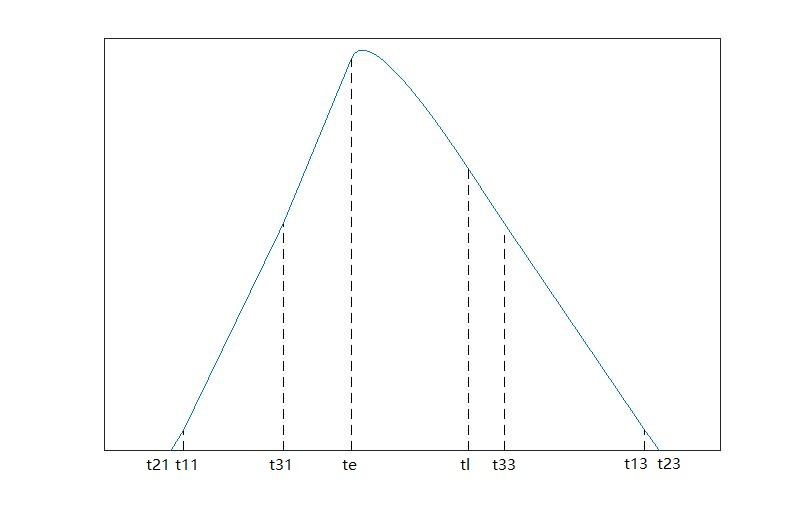
\includegraphics[width=3.5in]{image/case2.jpg}
	\caption{Queuing pattern at UE (General Case)}
	\label{fig:general case}
\end{figure}

Let $t_{i,1}$ and $t_{i,3}$ be the start and the end of departure times for mode $i$ ($i=1,2,3$). Known the queuing rate from Table \ref{tab:queuing rate} and the departure sequence, the queue length $Q_{i,j}(t)$ can be formulated as a continuous piece-wise function of departure time:

\begin{equation} \label{queuing length}
    Q_{i,j}(t)=\left\{
    \begin{array}{cl}
        Q_{2,1}\left(t\right)=\frac{s\beta}{\alpha+\mu_2-\beta}(t-t_{2,1}) & ,t\in\left[t_{2,1},t_{1,1}\right] \\
        Q_{1,1}\left(t\right)=\frac{s\beta}{\alpha+\mu_1-\beta}(t-t_{1,1})+Q_{2,1}\left(t_{1,1}\right) & ,t\in(t_{1,1},t_{3,1}] \\
        Q_{3,1}\left(t\right)=\frac{s\beta}{\alpha+\mu_3-\beta}(t-t_{3,1})+Q_{1,1}\left(t_{3,1}\right) & ,t\in(t_{3,1},t_e] \\
        Q_{3,2}\left(t\right)=-st+\sqrt{\frac{2A_3s^2}{B}\left(t-t_e\right)+\left[st_e+Q_{3,1}\left(t_e\right)-D_3\right]^2}+D_3 & ,t\in\left(t_e,t_l\right) \\
        Q_{3,3}\left(t\right)=\frac{-s\gamma}{\alpha+\mu_3+\gamma}(t-t_{3,3})+Q_{1,3}\left(t_{3,3}\right) & ,t\in[t_l,t_{3,3}) \\
        Q_{1,3}\left(t\right)=\frac{-s\gamma}{\alpha+\mu_1+\gamma}(t-t_{1,3})+Q_{2,3}\left(t_{1,3}\right) & ,t\in[t_{3,3},t_{1,3}) \\
        Q_{2,3}\left(t\right)=\frac{-s\gamma}{\alpha+\mu_2+\gamma}(t-t_{2,3}) & ,t\in\left[t_{1,3},t_{2,3}\right] \\
    \end{array}
    \right.
\end{equation}
where $A_3=\alpha+\mu_3$, $B=\frac{\beta+\gamma}{\bar{t}}$, $C=T_0-t^*$, $D_3=-s\left(\frac{A_3+\gamma}{B}+C\right)$.

Combining the general cost equation (\ref{GC eqaution}) and the queuing length (\ref{queuing length}), we can find out the start and end time of different mode road users respectively:

\begin{equation} \label{time point}
    \left\{
    \begin{array}{l}
        t_{2,1}=\frac{1}{\beta}\left[\left(\alpha+\mu_2-\beta\right)\left(T_0+\frac{\bar{t}}{2}\right)-GC_{MTR}\right]+t^* \\
        t_{1,1}=-\frac{GC_{MTR}}{\beta}+t^\ast+\frac{\delta\left(\alpha+\mu_2-\beta\right)}{\beta\left(\mu_2-\mu_1\right)} \\
        t_{3,1}=\frac{\delta-GC_{MTR}}{\beta}+t^\ast+\frac{\left(\tau-\delta\right)\left(\alpha+\mu_1-\beta\right)}{\beta\left(\mu_1-\mu_3\right)} \\
        t_e=t^*-\frac{\alpha+\mu_3-\beta}{\alpha+\mu_3}\times \frac{\overline{t}}{2}+\frac{\tau-GC_{MTR}}{\alpha+\mu_3} \\
        t_l=t^*+\frac{\alpha+\mu_3+\gamma}{\alpha+\mu_3}\times \frac{\overline{t}}{2}+\frac{\tau-GC_{MTR}}{\alpha+\mu_3} \\
        t_{3,3}=\frac{GC_{MTR}-\mu_0}{\gamma}+t^\ast-\frac{\left(\tau-\delta\right)\left(\alpha+\mu_1+\gamma\right)}{\gamma\left(\mu_1-\mu_3\right)} \\
        t_{1,3}=\frac{GC_{MTR}}{\gamma}+t^\ast-\frac{\delta\left(\alpha+\mu_2+\gamma\right)}{\gamma\left(\mu_2-\mu_1\right)} \\
        t_{2,3}=\frac{1}{\gamma}\left[GC_{MTR}-\left(\alpha+\mu_2+\gamma\right)\left(T_0+\frac{\bar{t}}{2}\right)\right]+t^\ast \\
    \end{array}
    \right.
\end{equation}

Then we can further derive the equilibrium flow of commuters with different mode:
\begin{equation}
    N_1=\frac{s\left(\beta+\gamma\right)}{\beta\gamma}\left[\frac{\left(\tau-\delta\right)\left(\alpha+\mu_1\right)}{\mu_1-\mu_3}-\frac{\delta\left(\alpha+\mu_2\right)}{\mu_2-\mu_1}+\delta\right]
    \label{N1}
\end{equation}
\begin{equation}
    N_2=\frac{s\left(\beta+\gamma\right)}{\beta\gamma}\left[\frac{\delta\left(\alpha+\mu_2\right)}{\mu_2-\mu_1}-\left(\alpha+\mu_2\right)\left(T_0+\frac{\bar{t}}{2}\right)\right]
    \label{N2}
\end{equation}
\begin{equation}
    N_3=\frac{2s\left(\beta+\gamma\right)}{\beta\gamma}\left[GC_{MTR}-\delta-\frac{\left(\tau-\delta\right)\left(\alpha+\mu_1\right)}{\mu_1-\mu_3}\right]
    \label{N3}
\end{equation}
\begin{equation}
    N_4=N-\frac{s\left(\beta+\gamma\right)}{\beta\gamma}\left[2GC_{MTR}+\delta-\left(\alpha+\mu_2\right)\left(T_0+\frac{\bar{t}}{2}\right)-\frac{\left(\tau-\delta\right)\left(\alpha+\mu_1\right)}{\mu_1-\mu_3}\right]
    \label{N4}
\end{equation}

So far, we got the equilibrium condition of the general case. However, during the peak period, not all the travel modes will be selected by the morning commuters, if the general cost of a certain mode is extremely higher. Typically, whether a travel mode is active depend on its time unit cost.

\begin{proposition}[Activation mode of taking taxi alone] \label{pro:positive N2}
    The non-sharing service will be used by commuters in the morning peak period, i.e. $N_2\geq{0}$, if and only if $\mu_2 \leq \mu_1+\frac{2\delta}{2T_0+\overline{t}}$
\end{proposition}
\textbf{Proof.} See the appendix.

Proposition \ref{pro:positive N2} indicates that time unit pricing $\mu_2$ can not be set beyond an upper bound limit otherwise no commuter prefers non-sharing service because its high price. In the upper limit condition, we can see the general cost of non-sharing service under free travel flow is the same as driving. However, it can't happen because during the peak period there must be congestion. Thus in the bottleneck, the general cost of non-sharing service will always be higher then driving. That is the reason why no one taking a taxi. Similarly, we can get the condition when mode of driving is active, seeing Proposition \ref{pro:positive N1}.

\begin{proposition}[Activation mode of driving] \label{pro:positive N1}
    The mode of driving during the morning peak hour will be utilized, i.e. $N_1 \geq{0}$, if and only if 
    
    (1) $\mu_1 \leq \mu_2-\frac{\delta}{\tau}(\mu_2-\mu_3)$, when mode of taxi is active;
    
    (2) $\mu_1 \leq \mu_3+\frac{2(\tau-\mu_0)}{2T_0+\overline{t}}$, when mode of taxi is inactive.
\end{proposition}
\textbf{Proof.} See the appendix.

Proposition \ref{pro:positive N1} implies the upper bound for the time-related pricing $\mu_1$ of driving. However, the time unit price of driving is determined by the level of gasoline consumption of the car, which is considered as an inherent factor. So if car is high in fuel consumption, no commuter will drive to work for its high cost. 

Both Proposition \ref{pro:positive N2} and \ref{pro:positive N1} show the positive ridership conditions of mode 1 and 2, indicating that even though relationship of the time-pricing parameters is assumed under Assumption \ref{ass:mu relation}, they can't be set beyond the upper bounds. 

As for ride-sharing service, with the lowest time-unit price, we assume that it won't be abandoned by commuters, otherwise it's worthless to study the equilibrium. To maintain ride-sharing service active in the bottleneck, the metro ticket price should be set higher than a lower bound value.

\begin{proposition}[Positive ridership of ride-sharing] \label{pro:positive N3}
    The mode of hailing ride-sharing car during morning peak period will be chosen, i.e. $N_3\geq 0$, if and only if $GC_{MTR}\geq \frac{\beta \overline{t}}{2}+\delta+\frac{\left(\tau-\delta\right)\left(\alpha+\mu_1\right)}{\mu_1-\mu_3}$
\end{proposition}
\textbf{Proof.} See the appendix.

Proposition \ref{pro:positive N3} indicates that the ride-sharing service will be terminated if the metro ticket fare is low enough. It is because ride-sharing service users, with relative low CVoT, are not so sensitive to their travel time. In another word, they prefer saving money rather than saving time. As a result, even though the travel time by metro is long, the ride-sharing users will be offset to take the metro if the ticket fee is low enough. 


\subsection{Sensitivity analysis of random travel delay}\label{subs:sensitivity test}

In the previous section, we discussed the general equilibrium conditions based on a given distribution of $R$ with the fixed maximum value $\overline{t}$, $R\sim U(0,\overline{t})$. But in reality, $\overline{t}$ is an expected value. If the road circumstances change, for example weather conditions and vehicle accidents, the travel delay is going to be different accordingly, and thus the equilibrium characteristics change. In this section, we conduct sensitivity analysis of $\overline{t}$ based on the general case to study how the random travel delay will affect the bottleneck performance in the morning peak period. 

\subsubsection{Active travel mode }\label{subsubs:Active travel mode}

With the travel delay varying, not all the three travel mode are available all the time. In general, with larger realization of random travel delay, less travel mode will be chosen. When $\overline{t}$ is high enough, violating Proposition \ref{pro:positive N2}, non-sharing service will be first abandoned by morning commuters. Similarly, mode of driving will be inactive when  Proposition \ref{pro:positive N1} is violated. Therefore, by shifting item with respect to $\overline{t}$ in Proposition \ref{pro:positive N2} and \ref{pro:positive N1}, we can get the relation between $\overline{t}$ and certain active travel modes on road. See Table \ref{tab:active mode}.

\begin{table}[htbp]
 \caption{Relation of random delay and active travel mode \label{tab:active mode}}
 \begin{center}
 \begin{tabular}{ccccc}
 
  \toprule
   $\overline{t}$ & driving & non-sharing service & ride-sharing service & metro \\
  \midrule
 $\left(0, \overline{t}_1 \right]$ & \checkmark & \checkmark & \checkmark & \checkmark \\
  $\left(\overline{t}_1, \overline{t}_2\right]$ & \checkmark &  & \checkmark & \checkmark \\
    $\left[\overline{t_2}, +\infty\right)$ & &  & \checkmark & \checkmark \\
  \bottomrule

 \end{tabular}
 \end{center}
Where $\overline{t}^0_1 = 2\left(\frac{\mu_0}{\mu_2-\mu_1}-T_0 \right)$ and $\overline{t}^0_2 = 2\left(\frac{\tau-\delta}{\mu_1-\mu_3}-T_0 \right)$.
\end{table}

Generally, larger value of $\overline{t}$ means that higher travel delay during the peak period. It indicates that all morning commuters have to spend more time on their trips. Since that, non-sharing service users, with the highest time-unit price, will have the largest increase amount of general cost. When the random travel delay reaches as large as $\overline{t}^0_1$, the expected cost using non-sharing service will be always higher than any other travel mode, and therefore no commuter will choose it. Similarly, no one will drive if $\overline{t}$ is higher than $\overline{t}^0_2$. 

In fact, by shifting term in Proposition \ref{pro:positive N3} we can get $\overline{t}$, i.e.  $\overline{t}^u = \frac{2}{\beta}\left[GC_{MTR}+\frac{\mu_0(\alpha+\mu_3)-\tau(\alpha+\mu_1)}{\mu_1-\mu_3} \right]$. When $\overline{t}$ is larger than $\overline{t}^u$, Proposition \ref{pro:positive N3} is violated and there will be no ride-sharing service in the bottleneck equilibrium. We don't consider such situation in our studies because the random travel delay can rarely be so large in reality. Thus, the upper bound of $\overline{t}$ is set to be $\overline{t}^u$.


\subsubsection{Total number of bottleneck vehicles $\overline{N}$}\label{subsubs:Total number of vehicles}
The vehicles on the road are inclusive of driving, non-sharing service and ride-sharing service cars.  One car is counted when commuters choose driving or non-sharing service, while two commuters share in one vehicle if they use ride-sharing service. Then based on equations \ref{N1}-\ref{N3}, the total number of vehicles $\overline{N}$ can be calculated:

\begin{equation}
\overline{N} =N_1+N_2+\frac{N_3}{2}
\end{equation}\label{Total number of vehicles}
To see the impact of $\overline{t}$ on $\overline{N}$, we take the partial derivative:
\begin{equation}
\frac{\partial \overline{N}}{\partial \overline{t}} = -\frac{s(\beta+\gamma)}{2 \beta \gamma}\left(\alpha+\mu_2 \right) < 0
\end{equation} \label{partial Nba}

Since the partial derivative is negative, the total number of vehicles of the bottleneck during the morning peak period will decrease when the random travel delay is getting larger. In this general case, 1 unit increase of $\overline{t}$ leads to  $\frac{s(\beta+\gamma)}{2 \beta \gamma}\left(\alpha+\mu_2 \right)$  unit deduction of vehicles on road,  more specifically, deduction of non-sharing service cars. That is because, seeing equations \ref{N1}-\ref{N3},  only $N_2$ is a function of $\overline{t}$. The quantity of driving and ride-sharing service remain unchanged before non-sharing service diminishes to be zero.  When it does, the amount of driving cars will decrease with the continuous growing $\overline{t}$. As the total amount of commuters in the morning peak period is fixed, the deduction part of car users will be absorbed by the metro system.

In another word, with the larger realization of random travel delay, more commuters are going to switch from on-road travel modes to metro. The users of non-sharing service will be first affected, and then the solo drivers. 


\subsubsection{Maximum queuing length $Q_{max}$}\label{subsubs: Maximum queuing length}
Equation \ref{queuing length} implies the cumulative length of queuing in the morning rush hour. In Figure \ref{fig:general case}, we can see that the cumulative queuing length before $t_e$ is linearly increasing, while it is linearly decreasing after $t_l$. Therefore, the maximum of queuing length must be gone through by the commuter that departs between $t_e$ and $t_l$. To obtain the maximum, we take the first-order partial derivative and set it to be zero:

\begin{equation*} 
\frac{\partial Q(t)}{\partial t} = 0 \Rightarrow t = t^\prime= t_e+\frac{\beta \overline{t}}{\beta+\gamma} - \frac{\beta^2 \overline{t}}{2(\alpha+\mu_3)(\beta+\gamma)}
\end{equation*}

Since $\frac{\partial^2 Q(t)}{\partial t^2} \geq 0$, the cumulative queuing length is a concave function of departure time. So, the maximum queuing length $Q_{max}$ is:

\begin{equation} \label{maximum queing length}
Q_{max} = Q(t^\prime) = s \left[\frac{\beta^2 \overline{t} }{2(\alpha+\mu_3)(\beta+\gamma)} - \frac{\alpha+\mu_3+\beta}{2(\alpha+\mu_3)}\overline{t} - \frac{\tau- GC_{MTR}}{\alpha+\mu_3} - T_0 \right]
\end{equation}

In the equation above, we know that the commuter starting his/her trip at time $t^\prime$ will go through the longest queuing time in the morning peak period. Furthermore, we take the partial derivative of equation \ref{maximum queing length} to do sensitivity analysis of $\overline{t}$:

\begin{equation} \label{partial Max Q}
\frac{\partial Q_{max}}{\partial \overline{t}} = -\frac{s}{2(\alpha+\mu_3)} \left(\alpha+\mu_3+\frac{\beta \gamma}{\beta+\gamma} \right) < 0
\end{equation}

The result shows that with 1 unit increment of $\overline{t}$, there is corresponding unit decrement of the maximum bottleneck queuing length. It is a counter-intuitive characteristic that larger random travel delay leads to a smaller maximum of queuing length. The reason is that, with higher travel delay on road, more commuters will choose metro instead of vehicles and thus less cars are operating during the peak period (see Section \ref{subsubs:Total number of vehicles}). Decreasing amount of vehicles on road means less congestion of the bottleneck. Therefore,  the peak of cumulative queuing length will decrease as well. 

\subsubsection{Total system queuing time $TQT$}\label{Total system queuing time}

In this section, we conduct analysis to see the total system queuing time with changing random delay. Graphically, it is shown in Figure \ref{fig:general case} as the square of the queuing pattern. Under different realization of the random delay, the change of the queuing pattern is shown in Figure \ref{fig:Queuing patterns with different random delay}.

\begin{figure}
	\centering
	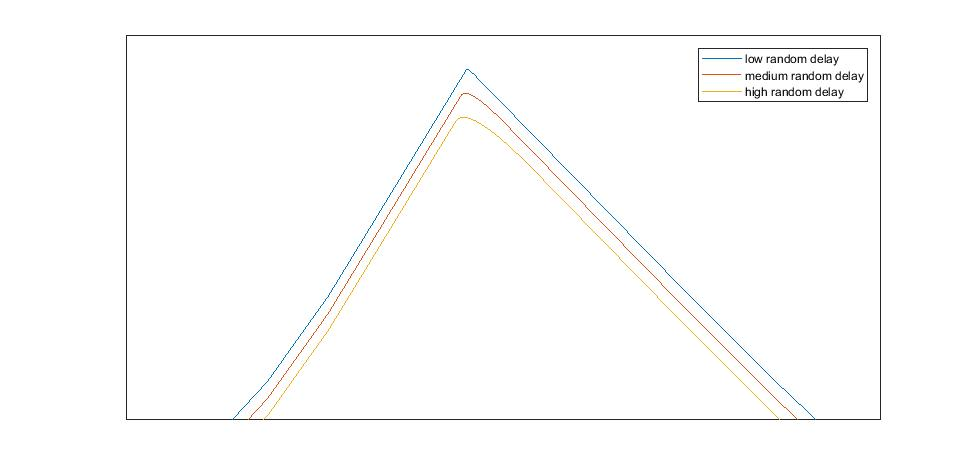
\includegraphics[width=3.5in]{image/QP_tba.jpg}
	\caption{Queuing patterns with different random delay}
	\label{fig:Queuing patterns with different random delay}
\end{figure}

In the figure, with the random delay growing higher, the square of the queuing pattern becomes smaller. In other words, the total system queuing time decreases. Analytically, the total system travel queuing time $TQT$ is defined as the integration of queue length $Q(t)$ over time $t$:

\begin{equation}
    TQT = \int^{t21}_{t11} Q(t) dt
\end{equation}

Then the $TQT-\overline{t}$ relationship is shown in Figure \ref{fig:Total queuing time under different random travel delay}. It is also a counter-intuitive property that high random delay has positive impact on the system queuing performance. In Section \ref{subsubs:Total number of vehicles}, we know, with higher realization of random travel delay, less vehicles are operating on the road during the morning peak period, making a less congested bottleneck. Therefore, the total system queuing time is shortened. 

Figure \ref{fig:Queuing patterns with different random delay} also shows that with the random travel delay becoming larger, the center of the bottleneck is becoming smoother. When random delay is low, there is an apparent peak in the center. The queue length on both sides of the peak is decreasing rapidly. When it is low, the peak is flattened. Departures in the bottleneck center will go through relatively same queuing length and there is no obvious culmination. 

\begin{figure}
	\centering
	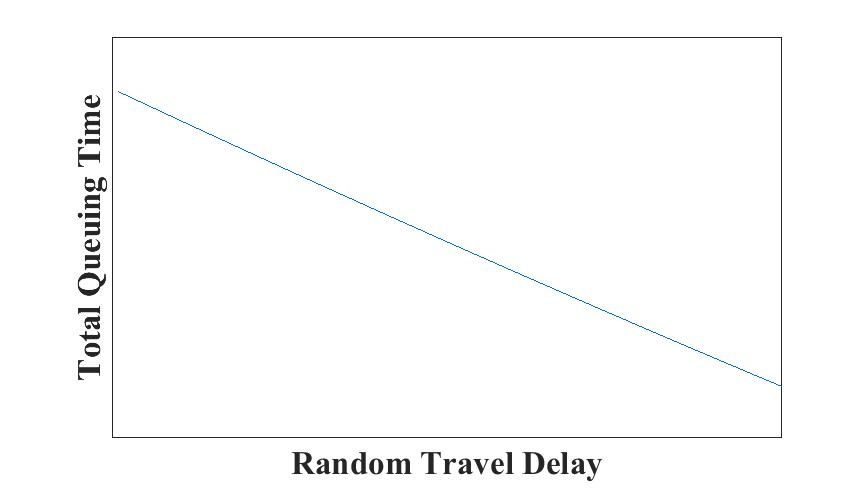
\includegraphics[width=3.5in]{image/TQT.jpg}
	\caption{Total queuing time under different random travel delay}
	\label{fig:Total queuing time under different random travel delay}
\end{figure}


\subsection{Impact of $\overline{t}$ and $GC_{MTR}$ on the on-time arrival status}\label{subs:impact on the on-time arrival status}

In the previous section, we discussed the general case with relatively low $\overline{t}$ and high $GC_{MTR}$ and only part of the ride-sharing service users are Type 2 commuters (not sure early or late arrival). Particularly, what travel mode users will be Type 2 commuters is determined by random travel delay $\overline{t}$ and the metro ticket fare $GC_{MTR}$. Moreover, these two essential factors also have impact on the queuing profile of the bottleneck. 

In this section, we analyze these two factors to how the queuing profile changes under different realization of them. However, it is hard to separate them up and analyze them one by one, because they affect the bottleneck simultaneously. Therefore, we analyze the impact considering $\overline{t}$ and $GC_{MTR}$ together at the same time.

Based on the relationship between $\overline{t}$ and active travel modes from Table \ref{tab:active mode}, there will be different travel modes available when $\overline{t}$ is within some certain intervals. Accordingly, we first classify all the cases into three categories with respect to $\overline{t}$, i.e.  $\left(0, \overline{t}^0_1 \right]$, $\left(\overline{t}^0_1, \overline{t}^0_2\right]$ and $\left[\overline{t^0_3}, +\infty\right)$. And then we analyze the impact in each category, considering $\overline{t}$ and $GC_{MTR}$ as continuous variables simultaneously. 

\textbf{Category One: $\overline{t} \in \left(0, \overline{t}^0_1 \right]$}

In this category, driving, non-sharing service and ride-sharing service are available on road as well as metro. Noticed that those who depart between time $t_e$ and $t_l$ are Type 2 commuters ($j=2$) And $\overline{t}$ is a main factor affecting the duration of the early-or-late time interval $(t_e,t_l)$. When $\overline{t}$ becomes larger, more commuters will become Type 2. But exactly which kind of commuters become Type 2 also depends on the setting of metro ticket fare $GC_{MTR}$. Based on this characteristic, we list out all the possible cases seeing Figure \ref{fig:Three-mode cases}.

\begin{figure}
	\centering
	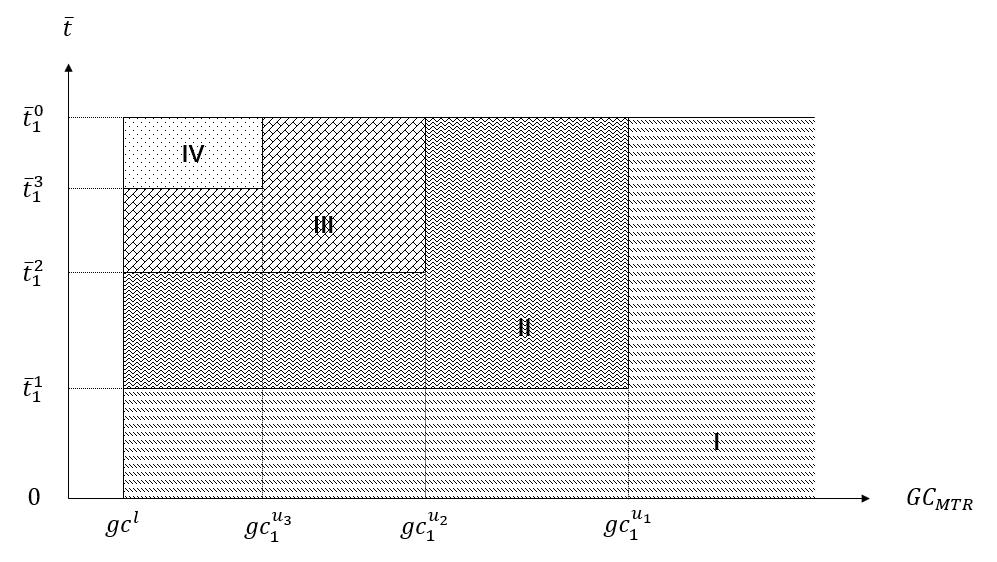
\includegraphics[width=3.5in]{image/Three-mode.jpg}
	\caption{Three modes on road}
	\label{fig:Three-mode cases}
\end{figure}

Case \uppercase\expandafter{\romannumeral1} is the general case as stated in Section \ref{subs:Equilibrium Condition}. In this case, no matter how $\overline{t}$ changes, only part of the ride-sharing service users are uncertain about their on-time arrival status. 
In Case \uppercase\expandafter{\romannumeral2}, the early-or-late time interval is inclusive of ride-sharing service users and part of drivers. Moreover, there won't be ride-sharing users who must be late at workplaces since they all depart before time $t_l$. 
Similarly, the early-or-late time interval in Case \uppercase\expandafter{\romannumeral3} includes all the three travel modes, and only those non-sharing service users depart after $t_l$ will be late certainly.
And in Case \uppercase\expandafter{\romannumeral4}, there will only two types of commuters: one who depart before $t_e$ must arrive early and the others who depart after $t_e$ are not sure whether they can be on time or not. And no one must arrive late.
%% expression for the points in Figure 2

Noticed that Figure \ref{fig:Three-mode cases} shows all the possible cases. However, not every case does exist in reality. $gc^{l}$ is regarded as the lower bound of $GC_{MTR}$ in order to make ride-sharing service as an active travel mode during the peak hour. Otherwise there won't be ride-sharing service in the market and we don't consider such situation in our study. As for the cut-off points on x-coordinate,  $gc_1^{u1}$, $gc_1^{u2}$ and $gc_1^{u3}$, they are functions of some given time unit pricing parameters respectively, the size relation among them can’t be confirmed straightforward. We can only prove that $ gc_1^{u3} < gc^{u2}_1 < gc_1^{u1}$, while the value of any of the three cut-off points may be less than $gc^{l}$ and therefore some of the potential cases may not show up in the figure. For example, for the given setting of time unit pricing parameters, if $gc_1^{u2}$ is calculated to be less than $gc^{l}$, i.e. the cut-off point $gc_1^{u2}$ moves to the left-hand side of $gc^{l}$, then the current Case  \uppercase\expandafter{\romannumeral3} and  \uppercase\expandafter{\romannumeral4} area will be covered by Case  \uppercase\expandafter{\romannumeral2}. As a result, there won’t be Case  \uppercase\expandafter{\romannumeral3} or  \uppercase\expandafter{\romannumeral4} in this situation regardless of $\overline{t}$ and $gc_{MTR}$.

Similarly, on y-coordinate, we have the relation $\overline{t}^1_1 < \overline{t}^2_1 < \overline{t}^3_1$ but we are not sure whether they lie in interval $\overline{t} \in \left(0, \overline{t}^0_1 \right]$ or not. If a certain cut-off point moves upward or downward, the relative case will prevail or be covered.

\textbf{Category Two: $\left(\overline{t}^0_1, \overline{t}^0_2\right]$}

\begin{figure}
	\centering
	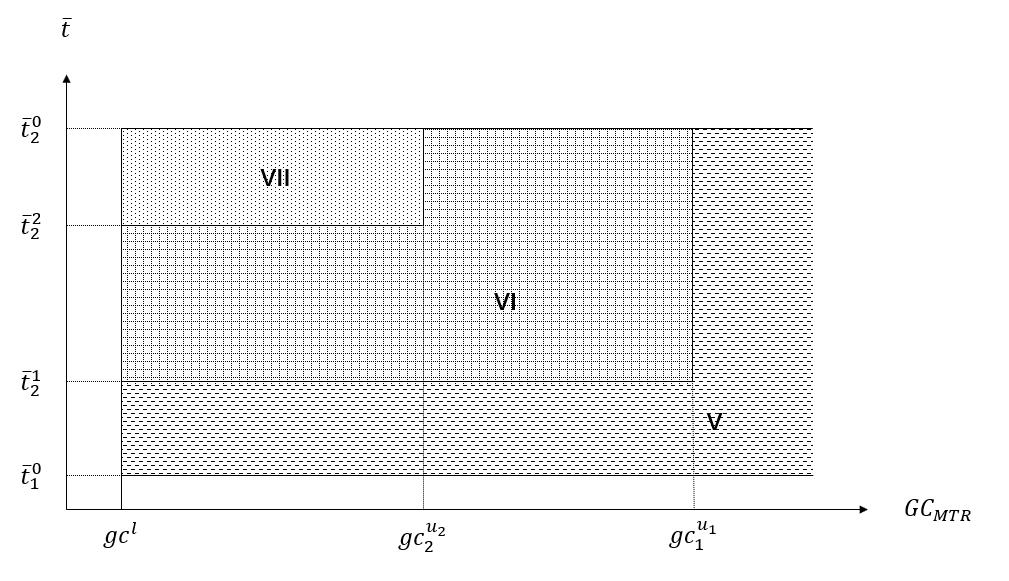
\includegraphics[width=3.5in]{image/Two-mode.jpg}
	\caption{Two modes on road}
	\label{fig:Two-mode cases}
\end{figure}

In this category, driving and ride-sharing service are available while non-sharing service is canceled in the morning peak period. Based on different on-time arrival status of commuters, the equilibrium can be classified into three cases, see Figure \ref{fig:Two-mode cases}.

The type of commuters in different cases is listed in Table \ref{tab:type of commuters 2 modes}. Similar as Category One, we only know $gc^{u2}_2 < gc_2^{u1}$ and $\overline{t}^1_2 < \overline{t}^2_2$. Whether $ gc^{u2}_2$, $gc_2^{u1}$ is larger than $gc^l$ or $\overline{t}^1_2$, $\overline{t}^2_2$ is higher than $\overline{t}^0_0$ is not sure. The actual case is determined by the given parameters in reality.
%% expressions 

\begin{table}[htbp]
 \caption{Type of commuters in different Case \label{tab:type of commuters 2 modes}}
 \begin{center}
 \begin{tabular}{cccc}
   \toprule
   Case & Type 1 & Type 2 & Type 3 \\
  \midrule
    \uppercase\expandafter{\romannumeral5} & driver, ride-sharing user & ride-sharing user & ride-sharing user, driver \\
    \uppercase\expandafter{\romannumeral6} & driver, ride-sharing user & ride-sharing user, driver & driver \\
    \uppercase\expandafter{\romannumeral7} & driver, ride-sharing user & ride-sharing user, driver & - \\
  \bottomrule
  
 \end{tabular}
 \end{center}
\end{table}



\textbf{Category Three: $\left[\overline{t^0_3}, +\infty\right)$}

\begin{figure}
	\centering
	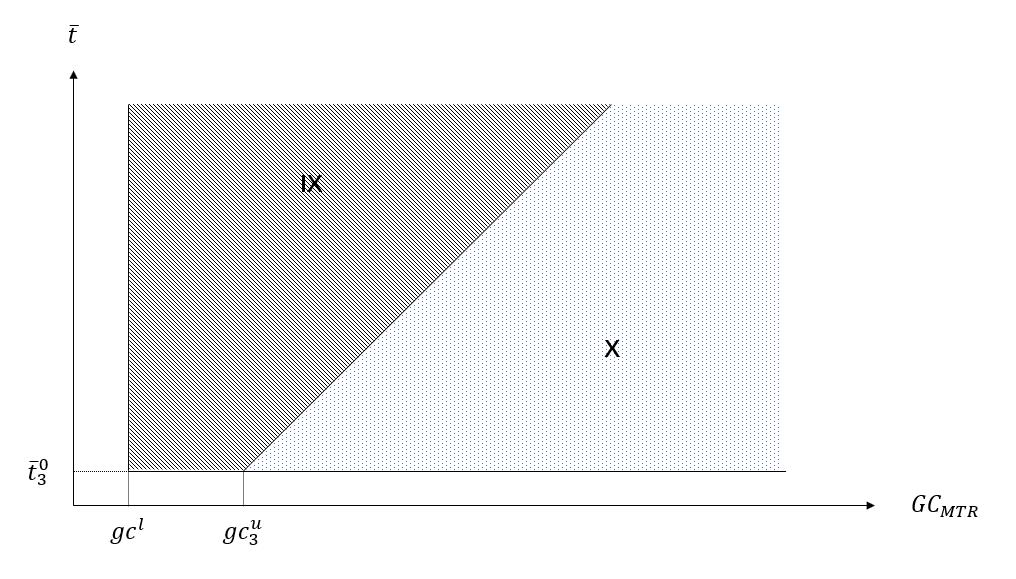
\includegraphics[width=3.5in]{image/One-mode.jpg}
	\caption{One mode on road}
	\label{fig:One-mode cases}
\end{figure}


\section{Numerical studies} \label{Numerical studies}




\section{Acknowledgements}
Gege Jiang is supported by General Research Fund \#615712 and \#616113 of the Research Grants Council of the HKSAR Government and the Hong Kong PhD Fellowship. Mogens Fosgerau is supported by the Danish Innovation Fund under the URBAN project.

\bibliographystyle{mf}
\bibliography{ref}

\appendix{}



\section{Appendix}

\begin{proof}[Proof of Proposition \ref{pro:positive N2}]

\noindent Sufficiency. Equation (\ref{N2}) shows the travel flow of single rider at UE. In order to keep it positive, we have
\begin{equation*}
    \frac{\delta\left(\alpha+\mu_2\right)}{\mu_2-\mu_1}-\left(\alpha+\mu_2\right)\left(T_0+\frac{\bar{t}}{2}\right) \geq 0
\end{equation*}
Known that $(\alpha+\mu_2)$ is positive, shifting item and then get the result.

\noindent Necessity. Given the proposition, by shifting we have 
\begin{equation*}
    \delta \geq(\mu_2-\mu_1)(T_0+\frac{\bar{t}}{2})
\end{equation*}
and since $\beta \geq{0}$, $\mu_2 >\mu_1$ and $\alpha+\mu_2-\beta \geq{0}$, then: 
\begin{equation*}
    -\frac{GC_{MTR}}{\beta}+t^\ast+\frac{\delta\left(\alpha+\mu_2-\beta\right)}{\beta\left(\mu_2-\mu_1\right)} \geq{\frac{1}{\beta}\left[\left(\alpha+\mu_2-\beta\right)\left(T_0+\frac{\bar{t}}{2}\right)-GC_{MTR}\right]+t^*}
\end{equation*}
yielding $t_{1,1} \geq{t_{2,1}}$. It implies that the start time of drivers lies after the start time of single riders. In another word, at least one of commuters choose to take a taxi alone.
\end{proof}

\begin{proof}[Proof of Proposition \ref{pro:positive N1}]

\end{proof}

\begin{proof}[Proof of Proposition \ref{pro:positive N3}] 

\noindent Sufficiency. Seen from Equation (\ref{N3}), to keep ride-sharing as an active travel mode in morning peak period, $N_3 \geq 0 $, we have $GC_{MTR}-\delta-\frac{\left(\tau-\delta\right)\left(\alpha+\mu_1\right)}{\mu_1-\mu_3} \geq 0$, then we get the lowest price setting of metro $gc^l$.

\noindent Necessity.  %free flow travel time
\end{proof}


\end{document}
